\documentclass[10pt,xcolor={table,dvipsnames},t]{beamer}
\usepackage{graphicx}
\usepackage{pgfgantt}
\setbeamercolor{title}{bg=ittol-blue,fg=white}
\setbeamercolor{frametitle}{bg=ittol-red,fg=white}

\title[Detección y reducción de falsos positivos en la clasificación de imágenes violentas contra la mujer]{\small
	INSTITUTO TECNOLÓGICO DE TOLUCA\\}

\author[Alumno: Francisco Primero Primero No. Control: M23281646 Asesor: Roberto Alejo]{\textcolor{Red}{\textbf{Detección y reducción de falsos positivos en la clasificación de imágenes violentas contra la mujer por medio de aprendizaje activo usando redes neuronales profundas}}}

\institute[]{\small Presentado por: Frank Prime \\
	No. de Control: 0000000 \\
	Asesor: Dr. R}
\date{\small Septiembre de 2024}

\begin{document}
	
	{
		\usebackgroundtemplate{
			\begin{picture}(320,55)
				\put(50,0){
\includegraphics[width=270pt,height=25pt]{figuras/logoSEP-TecNM-ITTol.png}}
				\institute{INSTITUTO TECNOLÓGICO DE TOLUCA}
			\end{picture}
		}
		\begin{frame}
			\titlepage
		\end{frame}
	}
	\begin{frame}{Tabla de Contenido}
		\tableofcontents
	\end{frame}
	
	\section{Antecedentes}
	\begin{frame}{Antecedentes}
		"A Deep Learning Approach to Detecting Gender-Based Violence in Social Media" Este artículo describe un enfoque de aprendizaje profundo para detectar la violencia de género en las redes sociales. El estudio utiliza una red neuronal convolucional (CNN) para clasificar las publicaciones de las redes sociales como violentas o no violentas. El estudio también utiliza un enfoque de aprendizaje activo para reducir el número de falsos positivos. \\ \\
		\begin{tikzpicture}
			\draw[->] (0,0) -- (5,0) node[right] {$x$};
			\draw[->] (0,0) -- (0,3) node[above] {$y$};
			\draw[blue, thick] (0,0) -- (1,1) -- (2,2) -- (3,1) -- (4,2) -- (5,3);
		\end{tikzpicture}
	\end{frame}
	
	\section{Planteamiento del Problema}
	\begin{frame}{Planteamiento del Problema}
		A pesar de su importancia, los árboles enfrentan amenazas como la deforestación, la urbanización y el cambio climático. Esto ha llevado a la disminución de la cobertura arbórea en muchas regiones. Es fundamental comprender cómo estos factores afectan a los árboles y desarrollar estrategias efectivas de conservación.
	\end{frame}
	
	\section{Fundamento Teórico}
	\begin{frame}{Fundamento Teórico}
		\begin{itemize}
			\item Los árboles desempeñan un papel vital en la captura de carbono a través de la fotosíntesis, ayudando así a mitigar el cambio climático.
			\item La diversidad de especies arbóreas es esencial para mantener la biodiversidad.
		\end{itemize}
		
		\begin{equation}
			\text{Cambio en la cobertura arbórea} = \text{Deforestación} - \text{Reforestación}
		\end{equation}
	\end{frame}
	
	\section{Hipótesis}
	\begin{frame}{Hipótesis}
		Nuestra hipótesis de investigación es que implementar programas de reforestación efectivos y promover la conservación de los árboles en áreas urbanas puede contrarrestar los efectos negativos de la deforestación y el cambio climático, aumentando la resiliencia de los ecosistemas forestales.
		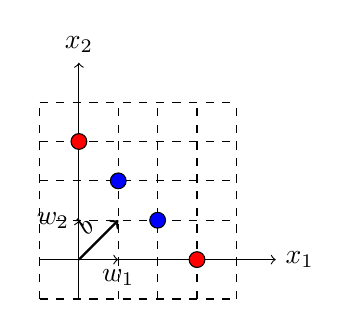
\begin{tikzpicture}[scale=0.5]
			\draw[->] (-1,0) -- (5,0) node[right] {$x_1$};
			\draw[->] (0,-1) -- (0,5) node[above] {$x_2$};
			\draw[dashed] (-1,-1) grid (4,4);
			\foreach \x/\y/\c in {0/3/red, 3/0/red, 1/2/blue, 2/1/blue} {
				\filldraw[fill=\c] (\x,\y) circle (0.2);
			}
			\draw[->] (0,0) -- (0,1) node[left] {$w_2$};
			\draw[->] (0,0) -- (1,0) node[below] {$w_1$};
			\draw[thick,->] (0,0) -- (1,1) node[midway,above,sloped] {$b$};
		\end{tikzpicture}
	\end{frame}
	
	\section{Justificación}
	\begin{frame}{Justificación}
		La investigación es fundamental debido a su relevancia para la conservación del medio ambiente y la calidad de vida de las comunidades urbanas. Comprender cómo los árboles afectan y son afectados por su entorno es esencial para tomar decisiones informadas en políticas de conservación y desarrollo sostenible.
		$$\int_{0}^{1} x^2 dx = \frac{1}{3}$$
	\end{frame}
	
	\section{Diseño de la Investigación}
	\begin{frame}{Diseño de la Investigación}
		\begin{itemize}
			\item Recopilación de datos de deforestación en áreas urbanas.
			\item Evaluación de programas de reforestación existentes.
			\item Análisis estadístico para determinar la correlación entre la cobertura arbórea y la calidad del aire en áreas urbanas.
		\end{itemize}
		
		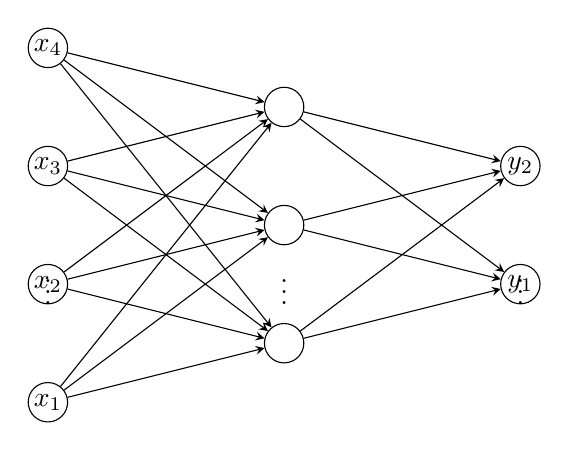
\begin{tikzpicture}[x=1.5cm, y=1.5cm, >=stealth]
			% Input layer
			\foreach \i in {1,...,4} {
				\node[circle, draw=black, fill=white, inner sep=0pt, minimum size=5mm] (I-\i) at (0,\i-2) {$x_\i$};
			}
			\node at (0,0) {$\vdots$};
			
			% Hidden layer
			\foreach \i in {1,...,3} {
				\node[circle, draw=black, fill=white, inner sep=0pt, minimum size=5mm] (H-\i) at (2,\i-1.5) {};
			}
			\node at (2,0) {$\vdots$};
			
			% Output layer
			\foreach \i in {1,...,2} {
				\node[circle, draw=black, fill=white, inner sep=0pt, minimum size=5mm] (O-\i) at (4,\i-1) {$y_\i$};
			}
			\node at (4,0) {$\vdots$};
			
			% Connections
			\foreach \i in {1,...,4} {
				\foreach \j in {1,...,3} {
					\draw[->] (I-\i) -- (H-\j);
				}
			}
			\foreach \i in {1,...,3} {
				\foreach \j in {1,...,2} {
					\draw[->] (H-\i) -- (O-\j);
				}
			}
		\end{tikzpicture}
	\end{frame}
	
	\section{Calendario de Actividades}
	\begin{frame}{Calendario de Actividades}
		\begin{table}
			\centering
			\begin{tabular}{|c|c|}
				\hline
				Mes & Actividad \\
				\hline
				Marzo & Recopilación de datos \\
				Abril & Análisis de datos \\
				Mayo & Evaluación de programas \\
				Junio & Redacción del informe \\
				Julio & Presentación de resultados \\
				\hline
			\end{tabular}
			\caption{Calendario de actividades de investigación}
		\end{table}
	\end{frame}
	
	\section{Cronograma}
	\begin{frame}{Cronograma}
		\begin{figure}[h]
			\centering
			
			\resizebox{\linewidth}{!}{%
				\begin{ganttchart}[
					y unit title=0.8cm,
					y unit chart=0.6cm,
					vgrid,
					hgrid,
					title label anchor/.style={below=-1.6ex},
					title left shift=.05,
					title right shift=-.05,
					title height=1,
					progress label text={},
					bar height=0.7,
					group right shift=0,
					group top shift=.6,
					group height=.3
					]{1}{16}
					%labels
					\gantttitle{Semestres}{16} \\
					\gantttitle{1}{4}
					\gantttitle{2}{4}
					\gantttitle{3}{4}
					\gantttitle{4}{4} \\
					%tasks
					\ganttbar[progress=100]{1. Revisión Bibliográfica}{1}{1} \\
					\ganttbar[progress=0]{2. Estado del Arte}{2}{8} \\
					\ganttbar[progress=0]{3. Protocolo}{2}{3} \\
					\ganttbar[progress=0]{4. Diseño de Experimento}{2}{5} \\
					\ganttbar[progress=0]{5. Colecciones de Datos}{3}{10} \\
					\ganttbar[progress=0]{6. Programación de Algoritmos}{5}{10} \\
					\ganttbar[progress=0]{7. Análisis de Resultados}{5}{11} \\
					\ganttbar[progress=0]{8. Presentación en Congreso}{6}{11} \\
					\ganttbar[progress=0]{9. Redacción de Artículo}{2}{12} \\
					\ganttbar[progress=0]{10. Escritura de Tesis}{2}{16} \\
				\end{ganttchart}%
			}
			\caption{Plan de Trabajo}
		\end{figure}
	\end{frame}
	
	\section{Referencias}
	\begin{frame}{Referencias}
		\begin{itemize}
			\item Smith, J. et al. (2019). Reforestation and its Impact on Urban Air Quality. \textit{Environmental Science Journal}, 45(2), 123-135.
			\item Brown, A. (2020). The Role of Trees in Climate Change Mitigation. \textit{Nature Reviews: Ecology and Evolution}, 18(3), 209-224.
		\end{itemize}
	\end{frame}
	
	\newpage
	
	\bibliography{bibliografia}									% Incluye la bibliografía contenida en el archivo "bibliografia.tex"
	\nocite{*}
	
\end{document}
